\chapter{Arbeitsgrundlagen}
% ==================================================================
\setcounter{page}{1} \thispagestyle{fancy} 
% ==================================================================
In diesem Versuch liegt das Hauptaugenmerk im Bereich der Schwingungen, welche in verschiedenen Gebieten der Physik vorkommen. Dabei wird konkret die \textbf{gedämpfte freie Schwingung}, sowie die \textbf{erzwungene Schwingung} betrachtet. Dafür wird ein Federpendel mit einer geschwindigkeitsproportionalen Reibung \\
%%%%%%%%%%%%%%%%%%%%%%%%%%%%%%%%%%%%%%%%%%%%%%%
\begin{equation}
F_{reib} = -\beta*v
\end{equation}
%%%%%%%%%%%%%%%%%%%%%%%%%%%%%%%%%%%%%%%%%%%%%%%
mit harmonischer Anregung \\
%%%%%%%%%%%%%%%%%%%%%%%%%%%%%%%%%%%%%%%%%%%%%%%
\begin{equation}
F_{anr}(t) = \hat{F}_{e}*cos(\omega*t)
\end{equation}
%%%%%%%%%%%%%%%%%%%%%%%%%%%%%%%%%%%%%%%%%%%%%%%
untersucht. Der Bremskoeffizient $\beta$ kann dabei als Konstant angenommen werden, da er durch die Anzahl, deren Abstände und Stärke der verwendeten Magneten (mehr dazu im Kapitel \ref{chap:durchfuehrung}) und von der Luftkissenbahn abhängt. Verbleiben diese also unverändert, ist $\beta$ konstant. Bei der harmonischen Anregung steht $\hat{F}_{e}$ für die Kraftamplitude und $\omega$ für die Erregerkreisfrequenz. \cite{w6}\\
\section{Gedämpfte freie Schwingung}
In der Abbildung \ref{fig:gedaempfteSchwingung} ist eine freie, gedämpfte Schwingung in zeitlicher Abhängigkeit zu sehen. \textit{T} entspricht der Periodendauer, welche trotz der Dämpfung konstant bleibt\footnote{siehe \textit{Eigenfrequenz} im Kapitel \ref{chap:begriffsexplikation}} 
und $x_{0}$ dem Wert von x(t) zum Zeitpunkt $t=0$.
%%%%%%%%%%%%%%%%%%%%%%%%%%%%%%%%%%%%%%%%%%%%%%%
\begin{figure}[h]
\centering
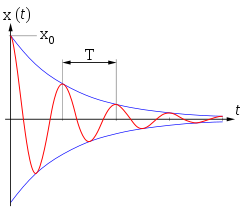
\includegraphics[scale=0.8]{Bilder/gedaempfte_schwingung.png}
\caption{Die Darstellung einer freien, gedämpften Schwingung im zeitlichen Verlauf x(t) \cite{freueSchw}}
\label{fig:gedaempfteSchwingung}
\end{figure}
%%%%%%%%%%%%%%%%%%%%%%%%%%%%%%%%%%%%%%%%%%%%%%%
\newpage
Mathematisch lässt sich diese Bewegung anhand der Gleichung \ref{equ:bewegung} beschreiben.
%%%%%%%%%%%%%%%%%%%%%%%%%%%%%%%%%%%%%%%%%%%%%%%
\begin{equation}
y(t) = \hat{y} * e^{-\Gamma*t} * cos(\omega*t-\delta)
\label{equ:bewegung}
\end{equation}
%%%%%%%%%%%%%%%%%%%%%%%%%%%%%%%%%%%%%%%%%%%%%%%
Dabei steht..
%%%%%%%%%%%%%%%%%%%%%%%%%%%%%%%%%%%%%%%%%%%%%%%
\begin{itemize}
	\item y(t) für die momentane, zeitabhängige Auslenkung des Fahrbahnpendels.
	\item $\hat{y}$ für die Auslenkung des Pendels zum Zeitpunkt $t=0$.
	\item $\Gamma$ für die Abklingkonstante.
	\item $\omega$ für die Kreisfrequenz des Federbahnpendels.
	\item $\delta$ für den Nullphasenwinkel der Schwingung.
\end{itemize}
\vspace*{0.5cm}
%%%%%%%%%%%%%%%%%%%%%%%%%%%%%%%%%%%%%%%%%%%%%%%
Die Ausklingkonstante $\Gamma$ lässt sich nach der Gleichung \ref{equ:gamma} berechnen.
%%%%%%%%%%%%%%%%%%%%%%%%%%%%%%%%%%%%%%%%%%%%%%%
\begin{equation}
\Gamma = \frac{\beta}{2*m}
\label{equ:gamma}
\end{equation}
%%%%%%%%%%%%%%%%%%%%%%%%%%%%%%%%%%%%%%%%%%%%%%%
Dabei giltet für $\omega$:
%%%%%%%%%%%%%%%%%%%%%%%%%%%%%%%%%%%%%%%%%%%%%%%
\begin{equation}
\omega = \sqrt{\omega_{0}^{2}-\Gamma^{2}}
\label{equ:omega}
\end{equation}
%%%%%%%%%%%%%%%%%%%%%%%%%%%%%%%%%%%%%%%%%%%%%%%
und für $\omega_{0}$:
%%%%%%%%%%%%%%%%%%%%%%%%%%%%%%%%%%%%%%%%%%%%%%%
\begin{equation}
\omega_{0}^{2} = \frac{k_{tot}}{m}
\end{equation}
%%%%%%%%%%%%%%%%%%%%%%%%%%%%%%%%%%%%%%%%%%%%%%%
$k_{tot}$ beschreibt die Gesamtfederkonstante, $m$ die Masse des Pendels und $\omega_{0}$ die Kreisfrequenz eines ungedämpften Pendels.
\section{Erzwungene Schwingung}
Eine erzwungene Schwingung kann wortwörtlich genommen werden. Das System wird in einer Erregerfrequenz harmonisch angeregt, wodurch eine Schwingung erzwungen wird. Je näher die Erregerfrequenz der Eigenfrequenz des schwingenden Pendels (oder allgemein des Systems) kommt, umso stärker schlägt die Amplitude aus. Deutlich zu erkennen ist dieses Phänomen in der Abbildung \ref{fig:erzwungeneSchwingung}.
%%%%%%%%%%%%%%%%%%%%%%%%%%%%%%%%%%%%%%%%%%%%%%%
\begin{wrapfigure}{r}{0.5\textwidth}
	\vspace{-20pt}
	\begin{center}
		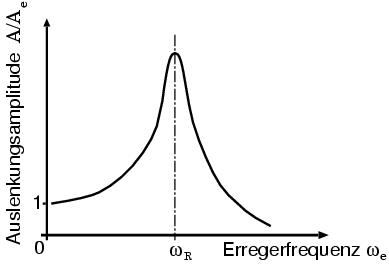
\includegraphics[scale=0.62]{Bilder/erzwungene_schwingung.png} 
	\end{center}
	\vspace{-20pt}
	\caption{Amplitudenresonanzkurve: das Amplitudenverhältnis in Funktion der Erregerfrequenz \cite{LP}. 		Bei zu niedriger Dämpfung könnte im schlimmsten Fall eine \textit{Resonanzkatastrophe} resultieren.}
	\label{fig:erzwungeneSchwingung}
	\vspace{-10pt}
\end{wrapfigure}
%%%%%%%%%%%%%%%%%%%%%%%%%%%%%%%%%%%%%%%%%%%%%%%
Nach der Gleichung \ref{equ:erzwungene} berechnet sich die Auslenkung der erzwungenen Schwingung. $\Omega$ beschreibt die Erregerkreisfrequenz. Umgerechnet zur Erregerfrequenz ergibt sich $f_{e} = \frac{\Omega}{2*\pi}$. Als $\hat{y}_{e}$ wird die Erregeramplitude bezeichnet. $k_{1}$ repräsentiert die Federkonstante der Erregerfeder.\\
%%%%%%%%%%%%%%%%%%%%%%%%%%%%%%%%%%%%%%%%%%%%%%%
\begin{equation}
\hat{y}(\Omega) = \frac{k_{1} * \hat{y}_{e}}{m*\sqrt{((\omega_{0}^{2}-\Omega^{2})^{2}+4*\Omega^{2}*\Gamma^{2})}}
\label{equ:erzwungene}
\end{equation}
%%%%%%%%%%%%%%%%%%%%%%%%%%%%%%%%%%%%%%%%%%%%%%%
Zur Berechnung der Phasenresonanz ergibt sich:
\begin{equation}
\delta=acos(\frac{\omega_{0}^{2}-\omega^{2}}{\sqrt{((\omega_{0}^{2}-\Omega^{2})^{2}+4*\Omega^{2}*\Gamma^{2})}})
\label{equ:phasenresonanz}
\end{equation}